\documentclass[english]{exercise}

\title{Homework 5}
\author{Joshua Feld (406718)}
\professor{Prof. Kowalski}
\course{Partial Differential Equations}

\begin{document}
    \maketitle


    \section{}

    \begin{quote}
        Consider the following one-dimensional boundary value problem
        \begin{align*}
            -u''\parentheses*{x} + u\parentheses*{x} &= f\parentheses*{x}, \quad \text{in }\parentheses*{0, 1} \subset \R,\\
            u\parentheses*{0} &= 0 \quad \text{(Dirichlet)},\\
            \alpha u\parentheses*{1} + u'\parentheses*{1} &= a, \quad \alpha \ge 0, a \in \R \quad \text{(Robin)}.
        \end{align*}
        \begin{enumerate}
            \item Derive the weak formulation of the above problem.
            \item Find the discrete solution using the finite element method.
            Choose the continuous piecewise linear functions
            \[
                \psi_i\parentheses*{x} := \begin{cases}
                    \frac{x - x_{i - 1}}{h_i}, & \text{if }x \in I_i = \parentheses*{x_{i - 1}, x_i},\\
                    \frac{x_{i + 1} - x}{h_{i + 1}}, & \text{if }x \in I_{i + 1} = \parentheses*{x_i, x_{i + 1}},\\
                    0, & \text{otherwise}
                \end{cases}
            \]
            as basis functions on a uniform grid, \(0 = x_0 < \cdots < x_N = 1\) with \(h = x_i - x_{i - 1}\).
        \end{enumerate}
    \end{quote}
    
    \begin{enumerate}
        \item
        \item
    \end{enumerate}
    
    
    \section{}
    
    \begin{quote}
        We again consider the one-dimensional Poisson problem
        \begin{align*}
            -u''\parentheses*{x} &= f\parentheses*{x}, \quad \text{in }\parentheses*{0, 1},\\
            u\parentheses*{0} = u\parentheses*{1} &= 0.
        \end{align*}
        The domain \(\Omega := \parentheses*{0, 1}\) is equipped with the grid \(0 = x_0 < \cdots < x_N = 1\).
        In contrast to the previous task, we now consider the approximation space \(V_h\) of continuous, piecewise quadratic functions, i.e.,
        \[
            V_h = \braces*{u \in C^0\parentheses*{\brackets*{0, 1}} : u_{\brackets*{x_{k - 1}, x_k}} = a_k + b_k x + c_k x^2, k = 1, \ldots, N, u\parentheses*{0} = u\parentheses*{1} = 0}.
        \]
        We equip this space with basis functions of the form displayed in Figure \ref{fig:2-1}.
        \begin{figure}[ht]
            \centering
            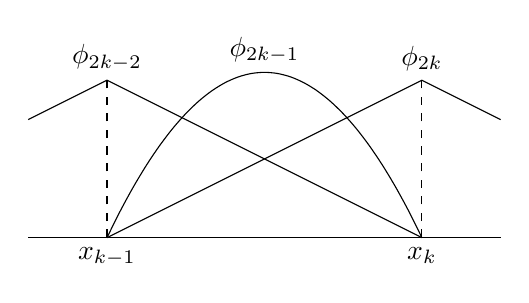
\begin{tikzpicture}
                \draw (0,0) -- (6,0);
                \node[anchor=north] at (1,0) {\(x_{k - 1}\)};
                \node[anchor=north] at (5,0) {\(x_k\)};
                \draw[dashed] (1,0) -- (1,2);
                \draw[dashed] (5,0) -- (5,2);
                \draw (0,1.5) -- (1,2) -- (5,0);
                \draw (1,0) -- (5,2) -- (6,1.5);
                \draw[domain=1:5, smooth, variable=\x] plot ({\x}, {-21/40*\x*\x + 63/20*\x - 21/8});
                \node[anchor=south] at (1,2) {\(\phi_{2k - 2}\)};
                \node[anchor=south] at (3,2.1) {\(\phi_{2k - 1}\)};
                \node[anchor=south] at (5,2) {\(\phi_{2k}\)};
            \end{tikzpicture}
            \caption{Piecewise quadratic basis functions}
            \label{fig:2-1}
        \end{figure}
        To be precise the basis consists of the usual \(N - 1\) hat functions \(\braces*{\phi_{2k}}_{k = 1}^{N - 1}\) together with an additional \(N\) functions \(\braces*{\phi_{2k - 1}}_{k = 1}^N\) defined as
        \[
            \phi_{2k - 1}\parentheses*{x} = \begin{cases}
                a + bx + cx^2, & \text{if }x \in \parentheses*{x_{k - 1}, x_k}\text{ with }\phi_{2k - 1}\parentheses*{\frac{x_{k - 1} + x_k}{2}} = 1,\\
                0, & \text{otherwise}.
            \end{cases}
        \]
        Write down the Galerkin discretization of this problem for the approximation space \(V_h\).
        Compute the stiffness matrix \(A\) using the definition of the basis \(\braces*{\phi_i}_{i = 1}^{2N - 1}\) of hat functions.
        Show your computations.
    \end{quote}
\end{document}
